\begin{figure}
    \centering
    \begin{subfigure}[b]{0.6\textwidth}
        \centering
        \includegraphics[width=\textwidth]{figs/figDiseasePoincare.png}
    \end{subfigure}
    \begin{subfigure}[b]{0.1\textwidth}
        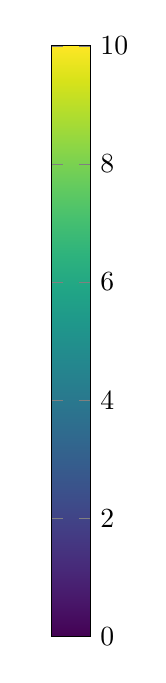
\begin{tikzpicture}
            \begin{axis}[
                hide axis,
                scale only axis,
                height=7.5cm,
                colorbar,
                colormap name=viridis,
                point meta min=0,
                point meta max=10,
                colorbar style={
                    height=7.5cm,
                    width=0.5cm,
                    ytick={0,2,...,10},
                    ticklabel style={fill=none, draw=none},
                    }      
                ]
                \addplot [draw=none, fill=none] coordinates {(0,0)};
            \end{axis}
        \end{tikzpicture}
    \end{subfigure}
    \label{fig:diseasePoincare}
    \caption{Shallow hyperbolic embeddings in the Poincaré disk of the \emph{Disease} hierarchical component. The color scale refers to the size of the neighbourhood of each node, in logarithmic scale.}

\end{figure}